% Originally: content/week-11.tex, \subsection{Green's theorem and conservative fields} --- promoted to a section

\section{Green's theorem and conservative fields}
\label{sec:greens_theorem_conservative_fields}

\begin{ainote}
Green's theorem, conservative vector fields, and path integrals were also discussed in the Monday session. 
\end{ainote}

\begin{theorem}[Green's Theorem]
\label{thm:greens_theorem}
Let $F : U \to \mathbb{R}^2$ be a continuously differentiable vector field on an open set $U \subseteq \mathbb{R}^2$. Then, for any compact $C^1$ domain $\Omega \subseteq U$,
\[\int_\Omega \curl F \mathop{d\text{vol}}_2 = \int_{\partial\Omega} F \cdot \tau \,dL,\]
where $\tau$ is the unit tangent vector to the boundary $\partial\Omega$ oriented counter-clockwise (i.e.\ $\tau = (-\nu_2, \nu_1)\transp$, with $\nu$ being the outward unit normal).
\end{theorem}

\begin{ainote}
% Supplement: Sascha Brack/Class Notes/Week_10_Notes_Monday.pdf, p. 16
\begin{center}
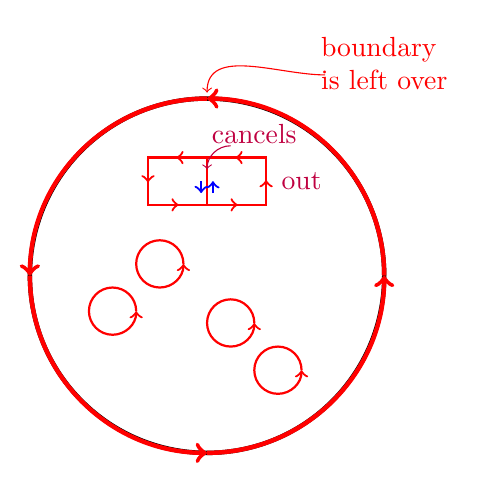
\begin{tikzpicture}[scale=1.5]
  % Domain
  \draw[ultra thick] (0,0) circle (1.5);
  % Boundary orientation
  \draw[red, ultra thick, ->] (1.5,0) arc (0:90:1.5);
  \draw[red, ultra thick, ->] (0,1.5) arc (90:180:1.5);
  \draw[red, ultra thick, ->] (-1.5,0) arc (180:270:1.5);
  \draw[red, ultra thick, ->] (0,-1.5) arc (270:360:1.5);
  
  \node[red, align=left] at (1.5, 1.8) {boundary\\is left over};
  \draw[red, ->] (1.0, 1.7) to[out=180, in=90] (0, 1.55);
  
  % Internal rotations
  \foreach \x/\y in {-0.6/-0.3, 0.4/-0.4, -0.2/0.1, 0.8/-0.8} {
    \draw[red, thick, ->] (\x,\y) arc (0:360:0.2);
  }
  
  % Two cancelling squares
  \draw[red, thick] (-0.5, 0.6) rectangle (0, 1.0);
  \draw[red, thick] (0, 0.6) rectangle (0.5, 1.0);
  % arrows
  \draw[red, thick, ->] (-0.25, 1.0) -- (-0.26, 1.0);
  \draw[red, thick, ->] (0.25, 1.0) -- (0.24, 1.0);
  \draw[red, thick, ->] (-0.5, 0.8) -- (-0.5, 0.79);
  \draw[red, thick, ->] (0.5, 0.8) -- (0.5, 0.81);
  \draw[red, thick, ->] (-0.25, 0.6) -- (-0.24, 0.6);
  \draw[red, thick, ->] (0.25, 0.6) -- (0.26, 0.6);
  
  \draw[blue, thick, ->] (-0.05, 0.8) -- (-0.05, 0.7);
  \draw[blue, thick, ->] (0.05, 0.7) -- (0.05, 0.8);
  
  \node[purple] at (0.4, 1.2) {cancels};
  \node[purple] at (0.8, 0.8) {out};
  \draw[purple, ->] (0.2, 1.1) to[out=180, in=90] (0, 0.9);
  
\end{tikzpicture}
\end{center}
We integrate the rotation inside the domain. Basically all the \qt{intermediate values} cancel out because for two points close to each other, the rotation points in opposite directions. Only the boundary is left over in the end!
\end{ainote}

\begin{example}[Area of a region via Green's theorem]
\label{ex:area_greens_theorem}
Consider a region $\Omega \subseteq \mathbb{R}^2$ defined by the region inside the curve $x^{2/3} + y^{2/3} = 1$ in the first quadrant, bounded by the axes. The curve can be parametrized as $\varphi(t) = (\cos^3 t, \sin^3 t)\transp$ for $t \in [0, \pi/2]$.

The area is $\vol_2(\Omega) = \int_\Omega 1 \mathop{d\text{vol}}_2$. We look for a vector field $F$ such that $\curl F = \partial_x F_2 - \partial_y F_1 \equiv 1$ on $\Omega$. A simple choice is $F(x,y) := (0, x)\transp$.
By Green's theorem, we have:
\[\vol_2(\Omega) = \int_\Omega \curl F \mathop{d\text{vol}}_2 = \int_{\partial\Omega} F \cdot \tau \,dL = \int_0^{\pi/2} F(\varphi(t)) \cdot \varphi'(t) \,dt.\]
Since $\tau(\varphi(t)) \,dL = \varphi'(t) \,dt$ along the parametrization, we compute the dot product:
\[F(\varphi(t)) \cdot \varphi'(t) = \begin{pmatrix} 0 \\ \varphi_1(t) \end{pmatrix} \cdot \begin{pmatrix} \varphi_1'(t) \\ \varphi_2'(t) \end{pmatrix} = \varphi_1(t)\varphi_2'(t).\]
This turns the area computation into a single 1D integral in $t$.
\end{example}

\begin{definition}[Conservative vector field]
\label{def:conservative_field}
Given a $C^k$ vector field $F$ on an open set $U \subseteq \mathbb{R}^n$, we call it \newterm{conservative} if there exists a scalar field $f : U \to \mathbb{R}$ of class $C^{k+1}$ such that $F \equiv \nabla f$. The function $f$ is called a \newterm{potential} for $F$.
\end{definition}

\begin{lemma}[Integrability conditions]
\label{lem:integrability_conditions}
Let $U \subseteq \mathbb{R}^n$ be open, and let $F$ be a $C^1$ conservative vector field on $U$ with components $F_1, \dots, F_n$. Then we necessarily have the integrability conditions:
\[\partial_j F_k = \partial_k F_j \qquad \text{for all } j, k \in \{1,\dots,n\}.\]
\end{lemma}
\begin{proof}
Let $f$ be a potential such that $F = \nabla f = (\partial_1 f, \dots, \partial_n f)\transp$. Then by Schwarz's theorem (symmetry of second derivatives),
\[\partial_j F_k = \partial_j(\partial_k f) = \partial_j\partial_k f = \partial_k\partial_j f = \partial_k(\partial_j f) = \partial_k F_j.\qedhere\]
\end{proof}

\begin{proposition}[Work along a path as difference of potential]
\label{prop:work_difference_potential}
Let $U \subseteq \mathbb{R}^n$ be open, and let $F : U \to \mathbb{R}^n$ be a continuous conservative vector field with potential $f$. Then for any $C^1$ path $\gamma : [0,1] \to U$, the line integral of $F$ along $\gamma$ depends only on the endpoints:
\[\int_\gamma F \cdot d\gamma = f(\gamma(1)) - f(\gamma(0)).\]
\end{proposition}
\begin{proof}
By definition of the path integral and the chain rule,
\begin{align*}
\int_\gamma F \cdot d\gamma &= \int_0^1 F(\gamma(t)) \cdot \gamma'(t) \,dt = \int_0^1 \nabla f(\gamma(t)) \cdot \gamma'(t) \,dt \\
&= \int_0^1 Jf(\gamma(t)) J\gamma(t) \,dt = \int_0^1 J(f \circ \gamma)(t) \,dt = \int_0^1 (f \circ \gamma)'(t) \,dt.
\end{align*}
By the fundamental theorem of calculus, this equals $(f \circ \gamma)(1) - (f \circ \gamma)(0) = f(\gamma(1)) - f(\gamma(0))$.
\end{proof}

\begin{example}[Line integral of a conservative field]
\label{ex:conservative_field_integral}
Consider the vector field $F : [0,1] \times [0,2] \to \mathbb{R}^2$ given by $F(x,y) := (y^2, 2xy)\transp$.
First, we show that $F$ is conservative by finding a potential $f$ such that $\nabla f = F$. We need $\partial_x f = y^2$ and $\partial_y f = 2xy$. Integrating the first equation with respect to $x$ gives $f(x,y) = xy^2 + c(y)$. Differentiating with respect to $y$ gives $\partial_y f = 2xy + c'(y)$, which must equal $2xy$. Thus $c'(y) = 0$, and we can choose $c(y) = 0$. The potential is $f(x,y) = xy^2$.

Now, let $\Gamma$ be a closed path on the boundary $\partial U$ of the domain, starting and ending at $\gamma(0) = \gamma(1) = (0,0)\transp$. By \cref{prop:work_difference_potential}, the line integral around this closed loop is simply the difference in potential at the endpoints:
\[\oint_\Gamma F \cdot d\gamma = f(\gamma(1)) - f(\gamma(0)) = f(0,0) - f(0,0) = 0.\]
\end{example}
